\documentclass[a4paper, 11pt]{scrreprt}
\usepackage[utf8]{inputenc}
\usepackage[T1]{fontenc}
\usepackage{lmodern}
\usepackage{amsmath,amssymb,amstext,amsfonts,mathrsfs, amsthm}
\usepackage{graphicx}
\usepackage{color}

\usepackage{marginnote}

\pagestyle{headings}

\newtheorem{defi}{Definition}[section]
\newtheorem{prop}[defi]{Proposition}
\newtheorem{theorem}[defi]{Theorem}
\newtheorem{coro}[defi]{Corollary}
\newtheorem{lemma}[defi]{Lemma}

\newcommand{\RR}{\mathbb{R}}
\newcommand{\EE}{\mathbb{E}}
\newcommand{\ZZ}{\mathbb{Z}}
\newcommand{\NN}{\mathbb{N}}
\newcommand{\FF}{\mathcal{F}}

\newcommand{\student}[1]{\marginnote{{\normalfont\bf #1}}}

\title{Abschlussarbeit Fallstudien der math. Modellbildung}
\author{Manuela Lambacher, Dominik Otto, Andreas Wiedemann}
\date{\today}

\begin{document}
\parindent 0pt
\maketitle
\tableofcontents

\chapter{Whittaker-Shannon Interpolation formula}

Sampling and reconstructing a signal from its samples are probably two of the most important properties of modern communication.   Even very simple things of our daily life, like making a phone call to our dear friend Massimo, are not possible without digitalizing analog signals, for example  our voice. \\
Whereas digitalizing can be done rather  straightforward by sampling, the real art is regaining the original signal from these samples or assessing the information lost in the sampling process.\\
In the following, we'd like to try to give a small survey of the famous Whittaker-Shannon interpolation formula, ist applications in real-life but also its limitations, keeping in mind the relationship of Fourier transform and the Heisenberg uncertainty principle.


\section{Preliminary notes and Sampling}
\begin{defi}[Fourier transform]
The Fourier transform \(\FF(f)\) of a d-dimensional, integrable function \(f:\RR^d \to \RR\) is given by
	\begin{equation}
		\FF f(w)=\int_{\RR^d} f(x)e^{-2\pi iwx}\,\mathrm{d}x
	\end{equation}

\end{defi}
So, the Fourier transform converts a time domain function into a frequency domain function. For example, the Fourier transform of an audio signal identifies the frequency spectrum as peaks in the frequency domain.\\
If \(\FF f\in L^1(\RR^d)\), then we can define the inverse Fourier transform:
\begin{defi}[Inverse Fourier transform]
\begin{equation}
	f(x) = \int_{\RR^d} \FF f(w) e^{2\pi iwx}\,\mathrm{d}w
\end{equation}
\end{defi}

\begin{defi}[bandlimited function]
	For \(Q = \prod_{i=1}^d \omega_i[-1/2, 1/2),\ \omega\in\RR^d\), we define
	\begin{equation}
		L_Q^2(\RR^d) = \{f\in L^2(\RR^d):\ supp(\FF f) \subset Q\}
	\end{equation}
	If \(f\in L_Q^2(\RR^d)\), then it is called \(\omega\)-bandlimited.
\end{defi}

\begin{lemma}[Bessel's inequality]
Let X be a Hilbert space, $S \subset X$ an orthonormal system. Then one has
\[\sum_{e \in S} |\langle x, e \rangle |^2 \leq \Vert x \Vert ^2\]
%Let X be a separable Hilbert space with $\dim(X) = \infty$ and $\{e_k:k \in \ZZ^d\}$ an orthonormal system. Then it is equivalent:
%\begin{itemize}
%\item[i)] $\{e_k:k \in \ZZ^d\}$ is an orthonormal basis
%\item[ii)] For all $x \in X$ Parseval's identity holds
%\[\Vert x \Vert^2 = \sum_{k\in \ZZ^d} |\langle x, e_k \rangle|^2\]
%\end{itemize}
\end{lemma}


\subsection{Sampling}
To convert a continuous function \(f\) into a sequence of discrete values is called sampling. In a mathematical way, sampling can be described as a multiplication of \(f\) with a dirac-comb 
\[s(t,\Delta T) = \sum_{n\in\ZZ} \delta(t-n\Delta T), \]
where \(\Delta T\) is the sampling intervall and \(\delta\) is the Dirac-function.\\
The sampled function \(\tilde{f}\) of our original \(f\) is denoted by
\begin{equation}
	\tilde{f} (t) = s(t,\Delta T) f(t) = \sum_{n\in\ZZ} f(t)\delta(t-n\Delta T)
\end{equation}
\begin{figure}[htpb]
	\centering
	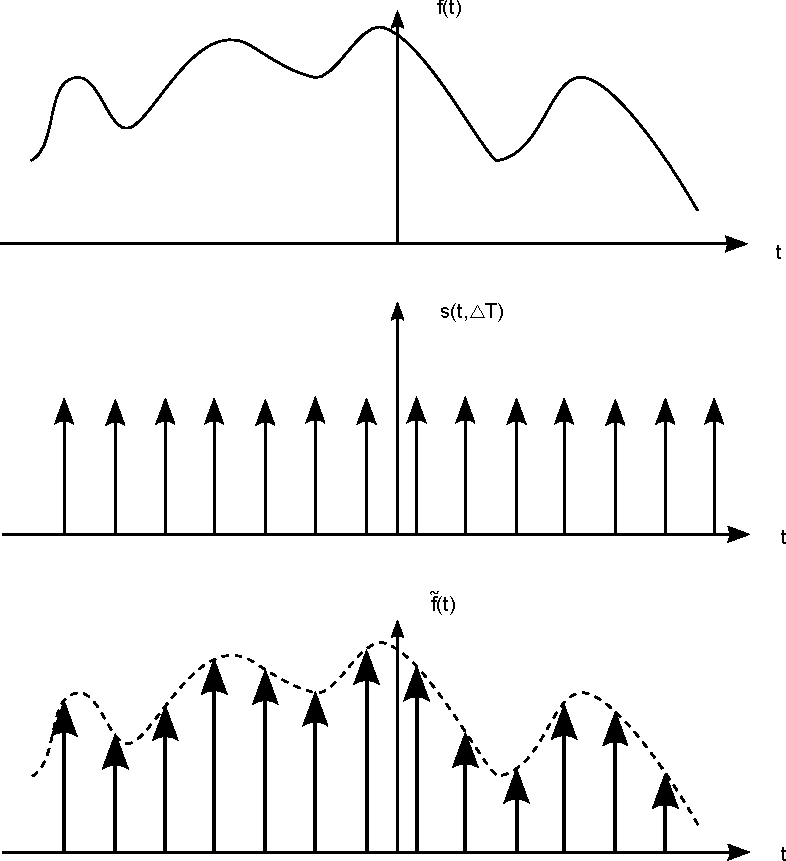
\includegraphics[width=0.65\textwidth]{Sampling-Visualisierung.pdf}
	\caption{(a) continuous function \(f\), (b) the dirac-comb, (c) sampled function as product of (a) and (b)}
\end{figure}
(see \cite{marks02})

The following theorem will be essential for our further work:
\begin{theorem}[perturbed sampling in \(L^2\)]
\label{th:perturbed sampling}
Let \(Q = \prod_{i=1}^d \omega_i[-1/2, 1/2)\) and \\
 \({f\in C(\RR^d)\cap L^2(\RR^d)}\) such that \(f_{|\tau\ZZ^d} \in l^2\). We write \(f=\eta + \epsilon\), where \(\FF\eta = \FF f\) on \(Q\). Then it holds
\begin{equation}
	f(x) = \sum_{k\in\ZZ^d} (f^c(\tau k)-\epsilon^c(\tau k))\prod _{i=1}^d sinc(\tau_i^{-1}x_i-k_i)+\epsilon(x), \qquad \text{in } L^2(\RR^d),
\end{equation}
where \(sinc(x) = \frac{sin(\pi x)}{\pi x}\).
\end{theorem}

\section{The Whittaker-Shannon Interpolation formula}

\begin{theorem}[Interpolation formula]
\label{th:interpolation}
If \(f \in L^2(\RR^d)\) is a \(\omega\)-bandlimited function, there exists a \(\tau_0 > 0\) such that for all \(\tau \in \left(0,\tau_0\right]\)
\begin{equation}
	f(x) = \sum_{k \in \ZZ^d} f^c(\tau k) \prod_{i=1}^d sinc\left(\tau_i^{-1} x_i -k_i\right).
\end{equation}
\end{theorem}
In other words, every bandlimited \(L^2\) function can be perfectly reconstructed from its samples, if the sampling rate is high enough! Holy Shit!\\
(Da der Beweis jetzt nicht mehr so umfangreich ist, ist ein eigenes Kapitel so viel denke ich, ich w"'urde ihn einfach direkt nach das Theorem setzen)\\
\begin{proof}[Proof]
We will prove the assertion by using theorem \ref{th:perturbed sampling}.\\ Let $f \in L^2(\RR^d)$ be a $\omega$-bandlimited function and set $\tau_0 := \frac{1}{\omega} = \left(\frac{1}{\omega_0}, \ldots, \frac{1}{\omega_d}\right)$ and $\epsilon := 0$. Besides choose $\tau \in (0,\tau_0]$ arbitrarily and define $T := \prod_{i=1}^d \left[-\frac{1}{2\tau_i} ,\frac{1}{2\tau_i}\right]$ and $Q := \prod_{i=1}^d \left[-\frac{1}{2}\omega_i ,\frac{1}{2}\omega_i\right]$.
\begin{itemize}
\item[i)] Since \(\FF(f)\) has a compact support and is continuous, $\FF(f)$ takes a maximal value $\Vert \FF(f) \Vert_\infty$. This leads to $\int_{\RR^d}| \FF f(w)|dw = \int_Q| \FF f(w)| dw \leq \Vert \FF(f) \Vert_\infty \mathscr{L}(Q) < \infty$. Therefore $\FF(f) \in L^1(\RR^d)$ and the fourier transform is reversible.
	 \[f(x) = \FF^{-1}(\FF(f))(x) = \int_{\RR^d}\FF(f)(\hat{x}) e^{2 \pi i (\hat{x},x)} d\hat{x}\]
	 Hence you can differentiate $f$.
	 \[df(x) = \left(\int_{\RR^d} \FF(f)(\hat{x}) e^{2 \pi i (\hat{x},x)} 2 \pi i \hat{x}_1 d\hat{x}, \ldots, \int_{\RR^d} \FF(f)(\hat{x}) e^{2 \pi i f t} 2 \pi i \hat{x}_d d\hat{x} \right)\]
	 You can easily see now that \(f \in C^\infty(\RR^d)\), thus $f \in C(\RR^d) \cap L^2(\RR^d)$.
\item[ii)] Now we want to show that $\{\det(\tau)^{d/2}\ e^{2 \pi i (w,k \tau)}\}_{k \in \ZZ^d}$ is an orthonormal system of $L^2(T)$.
\begin{align*}
\forall k,l \in \ZZ^d: \langle e_k(w), e_l(w) \rangle 
&= \det(\tau) \int_{T} e^{2 \pi i (\langle w,k \tau \rangle- \langle w,l \tau \rangle )}dw
= \det(\tau) \int_{T} e^{2 \pi i \langle w,(k-l) \tau \rangle}dw \\
&= \int_{-\frac{1}{2\tau_1}}^{\frac{1}{2\tau_1}} \cdots \int_{-\frac{1}{2\tau_d}}^{\frac{1}{2\tau_d}} \prod_{j=1}^d \tau_j e^{2 \pi i w_j (k_j-l_j) \tau_j}dw_1 \ldots dw_j \\
&= \prod_{j=1}^d \int_{-\frac{1}{2\tau_j}}^{\frac{1}{2\tau_j}} \tau_j e^{2 \pi i w_j (k_j-l_j) \tau_j}dw_j
\end{align*}

If $k \neq l$, then there is a $j \in \{1,\ldots,d\}$ such that $k_j \neq l_j$. With regard to the integral, it means:

\begin{align*}
\int_{-\frac{1}{2\tau_j}}^{\frac{1}{2\tau_j}} \tau_j e^{2 \pi i w_j (k_j-l_j) \tau_j}dw_j
&= \left[ \frac{1}{2 \pi i (k_j - l_j)} e^{2 \pi i w_j (k_j-l_j) \tau_j} \right]_{w_j = -\frac{1}{2 \tau_j}}^{\frac{1}{2 \tau_j}} \\
&= \frac{1}{2 \pi i (k_j-l_j)} \left( e^{\pi i (k_j-l_j)} - e^{-\pi i (k_j-l_j)} \right) = 0
\end{align*}

In case $k = l$ we can conclude:
\[\prod_{j=1}^d \int_{-\frac{1}{2\tau_j}}^{\frac{1}{2\tau_j}} \tau_j e^{2 \pi i w_j (k_j-l_j) \tau_j}dw_j
= \prod_{j=1}^d \tau_j \left(\frac{1}{2\tau_j}+\frac{1}{2\tau_j}\right) = 1\]

Consequently $\{\det(\tau)^{d/2}\ e^{2 \pi i (w,k \tau)}\}_{k \in \ZZ^d}$ is an orthonormal system of $L^2(T)$. (It is even an orthonormal basis.)

That's why one has Bessel's inequality.
\begin{align*}
\sum_{k \in \ZZ^d} |f(k \tau)|^2
&= \sum_{k \in \ZZ^d} | \int_{\RR^d} \FF f(w) e^{2 \pi i \langle w,k \tau \rangle}dw|^2 \\
&= \sum_{k \in \ZZ^d} | \left\langle \FF f(w), e^{2 \pi i \langle w,k \tau \rangle}\right\rangle |^2
\leq (\det(\tau))^{-d} \Vert \FF f \Vert_{L^2(T)}^2 < \infty
\end{align*}
So the condition $f_{|\tau\ZZ^d} \in l^2$ is fulfilled.

\end{itemize}

So theorem \ref{th:perturbed sampling} is applicable and we can conclude:
\begin{align*}
f(x) &= \sum_{k\in\ZZ^d} (f^c(\tau k)-\epsilon^c(\tau k))\prod _{i=1}^d sinc(\tau_i^{-1}x_i-k_i)+\epsilon(x) \\
&= \sum_{k \in \ZZ^d} f^c(\tau k) \prod_{i=1}^d sinc\left(\tau_i^{-1} x_i -k_i\right)  
\end{align*}

\end{proof}
\begin{figure}[htpb]
	\centering
	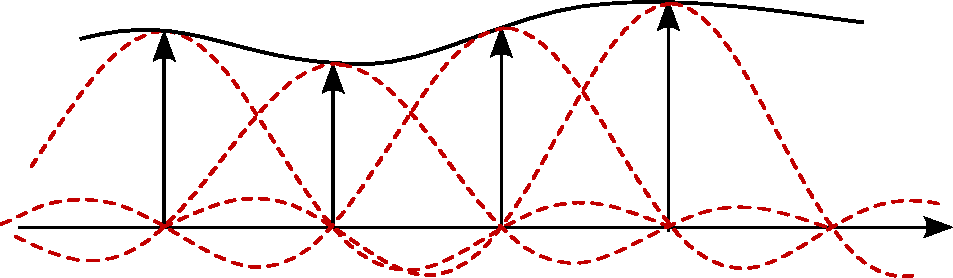
\includegraphics[width=0.80\textwidth]{Rekonstruktion-Visualisierung.pdf}
	\caption{Visualisation of the interpolation formula for \(d=1\): the original signal (black line) is reconstructed by weighted and shifted sinc-functions}
\end{figure}

\section{Meaning, real-life applications and limitations}

\subsection{Meaning}

Now we know, that a band-limited \(L^2\) function can be perfectly reconstructed with \(\tau_0\) small enough. Indeed, it is possible to determine \(\tau_0\) more precisely:
\begin{theorem}[Shannon-Nyquist sampling theorem]
\label{th:sampling}
Let \(f\in L^2_Q(\RR^d)\), \(\lambda_{max}\) the highest frequency of \(f\), \(\frac{1}{\tau}\in \RR^d\) the sampling rate. If \(\frac{1}{\tau_0} \geq 2\cdot \lambda_{max}\), \(f\) can be reconstructed from its samples for all \(\tau \leq \tau_0\).\\
\(\frac 1 2 \frac{1}{\tau_0}\) is called the Nyquist-rate or Nyquist-frequency.
\end{theorem} 
\begin{proof}
See \cite{shannon01}.
\end{proof}
(den Beweis abzuschreiben waere gar zu klaegliche Platzverbraucherei oder? ;))\\
\textbf{Remark:} The Whittaker-Shannon interpolation formula (Theorem  \ref{th:interpolation}) and the Shannon-Nyquist sampling theorem (Theorem \ref{th:sampling}) are often combined as the "Shannon-Nyquist-Whittaker sampling theorem".\\
The problem with Theorem  \ref{th:interpolation} and Theorem \ref{th:sampling} is that they are highly theoretical and could only be used in an ideal environment. The perfect reconstruction of a signal is not possible, since we would need infinitely many sampling points. But we can interpolate the original signal with arbitrary precision, if we just add enough sampling points. This is true because \(f(t)\to 0\) for \(t\to\pm\infty\), since \(f\in L^2\). So there is an Intervall \(I\) outside of which the samples are basically 0. If we sample over \(I\) at the Nyquist rate (or higher), the signal is characterized well enough, for \(I\) sufficiently large. (see \cite{marks02})\\
Even worse, Theorem  \ref{th:interpolation} and Theorem \ref{th:sampling} cannot be used for discontinuous signals or periodical signals, which are not in \(L^2\). As we will see later (see section \ref{se:uncertainty} Uncertainty principle), they even can't be used for finite signals, because finite signals are not bandlimited. \\
With these restrictions, the theorems seem to be of only small use in real life, but in section \ref{se:real-life} we will see the potential sleeping in them.\\
(zumindest hoffe ich das)


\subsection{Uncertainty Principle}
\label{se:uncertainty}
Warum haben wir das nur fuer d=1 gemacht??
\begin{theorem}[Uncertainty principle]
Let \(g\in L^2(\RR) \) and \(a,b \in\RR\) two arbitrary scalars. Then
\begin{equation}
\label{eq:uncertainty}
\left(\int_{\RR} (x-a)^2|g(x)|^2 \,\mathrm{d}x\right)\left(\int_{\RR}(\omega-b)^2|\FF g(\omega)|^2\,\mathrm{d}\omega\right) \geq \frac{||g||_2^2}{4\pi}
\end{equation}
\end{theorem}
(die hoch 1/2 im Skript sind falsch denke ich)\\
Which means, that an analyzing function (window) cannot be arbitrarily concentrated in the time- and frequency-domain at the same time. So a signal with compact support is not bandlimited, whereas a bandlimited signal can't be compactly supported (in particular not finite).\\
If \(g\) is a Gaussian function, then it holds 
	\[\left(\int_{\RR} (x-a)^2|g(x)|^2 \,\mathrm{d}x\right)\left(\int_{\RR}(\omega-b)^2|\FF g(\omega)|^2\,\mathrm{d}\omega\right) = \frac{||g||_2^2}{4\pi}\]
So the Gaussian is the function with minimal uncertainty/  which is equally concentrated in time and frequency. This property of the Gaussian function is used for example in image editing via the Gaussian filter, which is smoothing parts of a picture. (Steht bei Wikipedia, aber eine Quelle, wo der Zusammenhang mathematisch erlaeutert wird, finde ich leider nicht)\\
If \(g\in L^2(\RR^d)\) with \(||g||_2=1\), then, because of the Plancherel equality \(||g||_2=||\FF g||_2\), both \(|g|^2\) and \(|\FF g|^2\) are probability distributions on \(\RR^d\). With \(a=mean(g)\) and \(b=mean(\FF g)\), (\ref{eq:uncertainty}) can be written as
	\[var|g|^2 \cdot var|\FF g|^2 \geq \frac{1}{4\pi},\]
the famous Heisenberg uncertainty principle!\\	
Physically, this result says that position distribution and momentum distribution of a quantum particle cannot be sharply peaked at the same time. Mathematically, one can say that position and momentum are Fourier transforms of one another.\\
If we return to our example of audio signals, (\ref{eq:uncertainty}) can be understood in the following way:\\
If the signal \(f\) ist very short, it is not possible to determine the frequencies \(\lambda\) exactly, while on the other hand sound at one exact frequency corresponds to a perfect sine wave with no beginning or ending.

\subsection{Real-Life Applications}
\label{se:real-life}

\subsubsection{Audio signals}
Normal audio signals, for example music or voice recordings, are rather "nice" functions because of their continuity. Besides, the human hearing is rather bad in comparison to that of many animals, which allows us to execute some simplifications:\\
Earlier we mentioned that finite signals are not bandlimited. But in this special case we don't have to operate with frequencies below 20 Hz or above 20 kHz, since we can't hear them. So if we "cut off" the frequencies outside our hearable frequency range, we don't lose significant information and achieve the signal to be bandlimited. So by Theorem \ref{th:interpolation}, we can reconstruct such prepared signals with arbitrary precision. \\
(Sollen wir hier noch weiter auf Komprimierungsmoeglichkeiten eingehen? Finde ich recht interessant, hat aber nicht wirklich was mit dem Thema zu tun...)


\nocite{marks02}
\nocite{fornasier03}

\bibliography{literature}
\bibliographystyle{plain}
\end{document}
